This chapter offers an overview of the different implementation steps to develop the project.

\section{System Architecture Overview}

Follow low-level implementation detail of the different stages of the pipeline.\\

Include code snippets for individual sections.

\begin{figure}[h] 
\centerline{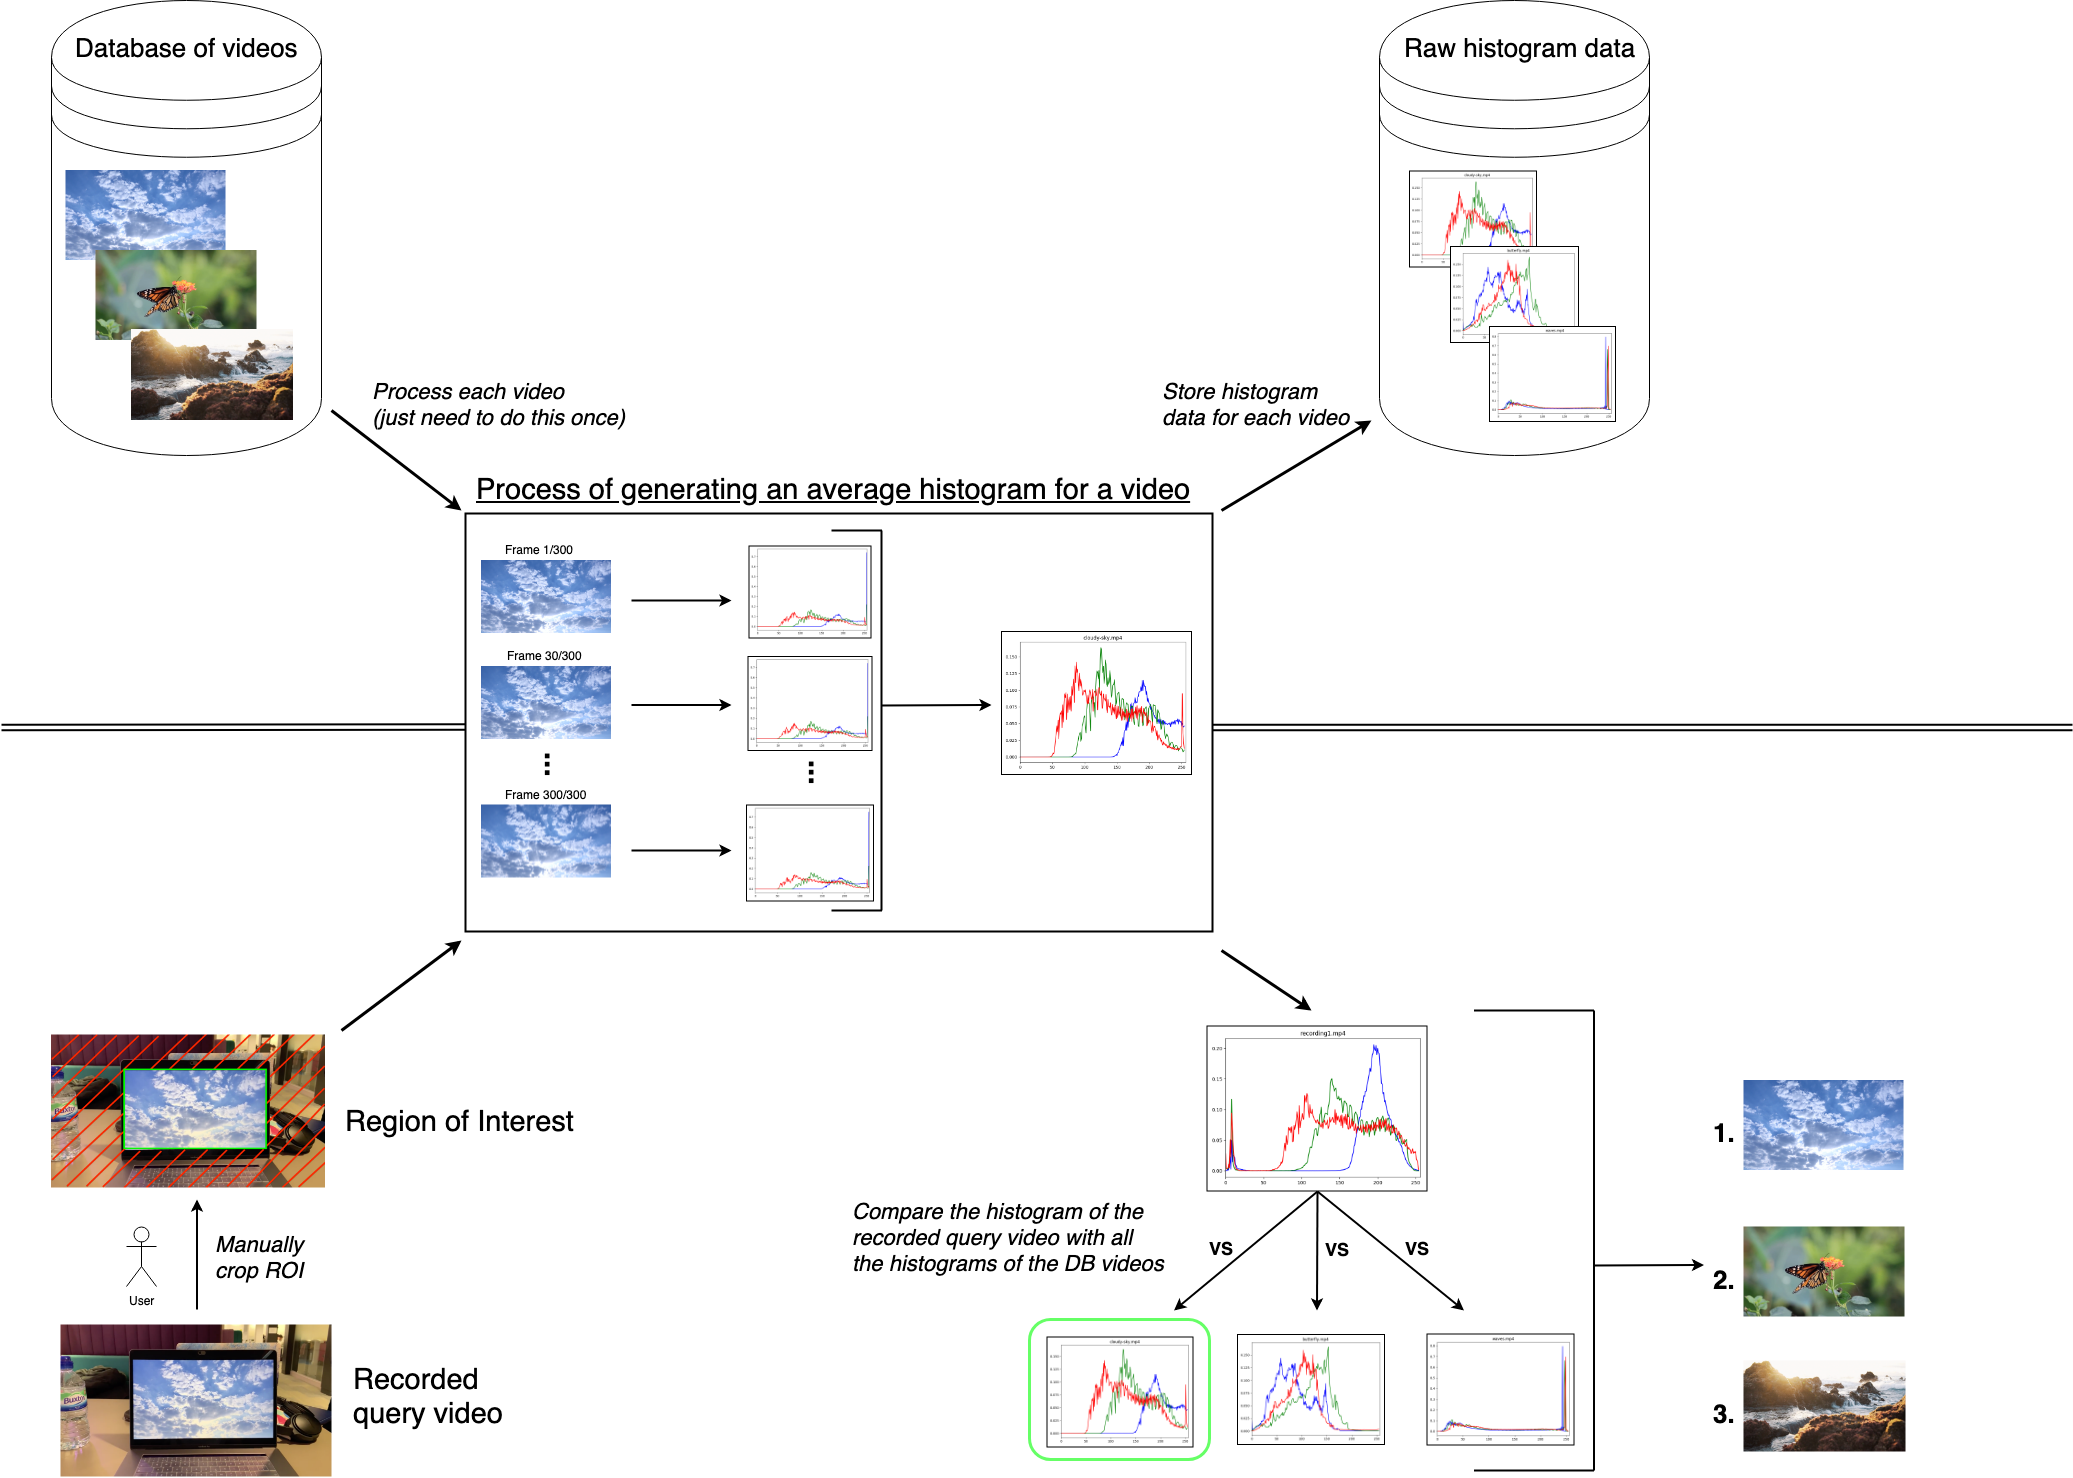
\includegraphics[width=\textwidth]{figures/implementation/CBVR-flowchart.png}}
\caption{\label{fig:CBVR flowchart}Flowchart.}
\end{figure}

\section{Offline Colour-Based Feature Extraction}

\subsection{RGB Histogram Generation}

An RGB histogram is generated for each database video. 

\begin{itemize}
    \item generating RGB histograms
    \item generating greyscale histograms
    \item generating HSV histograms
    \item averaging histogram
    \item histogram normalisation
    \item saving data to human-readable .txt files
\end{itemize}

\section{Online Retrieval}

\begin{itemize}
    \item query video, identical features extracted, video stabilised
    \item distance measurements to find nearest neighbour between query histograms and each database video histogram:
        \begin{itemize}
            \item correlation
            \item intersection
            \item chi-square
            \item alternative chi-square
            \item bhattacharyya
            \item kullback leibler divergence
            \item wassertein distance (Earth's Mover Distance)
            \item energy distance
        \end{itemize}
    \item combining results from all 3 methods with weight between different histogram methods to give more importance to HSV, GRB and less importance to grey scale: 1-5-10
\end{itemize}

\section{Database Pre-Processing}

\begin{itemize}
    \item shot boundary detection for long videos, allowing the entire movie to be represented with a few thousand frames
    \item current: one frame every second for short videos
\end{itemize}

\section{Output-Related}

\begin{itemize}
    \item opencv box drawing to select Region of Interest
    \item matplot lib histogram plotting (with an option to show each generated histogram or to hide them)
    \item tables to show scores for each type of histogram and each distance
    \item exporting results to CSV for further analysis
    \item spinners to show calculations are being done when training the system or stabilising videos 
    \item argument parsing
    \item final output to clearly show if result if right/wrong, including a frame of the original query video, a frame of the match found, along with the runtime and tha accuracy
\end{itemize}

\section{Testing}

\begin{itemize}
    \item Unit Testing
        \begin{itemize}
            \item grey scale / RGB / HSV histogram generation
            \item histogram saving to file
            \item histogram normalisation
            \item ROI selection
            \item individual histogram matching, test each metric
        \end{itemize}
    \item Integration Testing
        \begin{itemize}
            \item test the entire pipeline (with a few videos as the database, make sure the correct match is found)
        \end{itemize}
    \item Include some code snippets
    \item Include test suite results
\end{itemize}